\documentclass{beamer}

\usepackage[francais]{babel}
\usepackage[T1]{fontenc}
\usepackage[utf8]{inputenc}
\usepackage{beamerthemecs}
\usepackage{beamerouterthemecs}
\usepackage{beamerfontthemecs}
\usepackage{beamerinnerthemecs}
\usepackage{beamercolorthemecs}

\usetheme{cs}
\useoutertheme{cs}
\usefonttheme{cs}
\useinnertheme{cs}
\usecolortheme{cs}

\title[Les Réseaux Zigbee]{Les Réseaux Zigbee}
\author{\textbf{Thibault \textsc{Lengagne}, Sofian \textsc{Medbouhi} et Staninslas \textsc{Fechner}}}
\institute{Centrale Supélec - Campus de Rennes}

\begin{document}

  \begin{frame}
    \titlepage
  \end{frame}
  
  \AtBeginSection[] {
    \begin{frame}
      \frametitle{Plan}
      \tableofcontents[currentsection, hideothersubsections, pausesubsections]
    \end{frame} 
  }

\section{Introduction}
  \begin{frame}
   \frametitle{Zigbee, IEEE 802.15.4 et LR WPAN}
   \begin{block}{Zigbee IEEE 802.15.4}
   \begin{itemize}
	   \item IEEE 802.15.4 définit les couches basses (physique et mac)
	   \item Zigbee définit les couches réseau et applicative
	   \item Cependant Zigbee fonctionne toujours sur 802.15.4, on confond souvent les deux..
   \end{itemize}
   \end{block}
  \end{frame}

\begin{frame}
   \frametitle{Fonctions principales}

   \begin{block}{\textit{Zigbee} doit permettre de construire un réseau avec des équipements}
   \begin{itemize}
    \item de faible consommation
    \item de faible débit/portée
    \item de faible puissance (de calcul)
   \end{itemize}
   Ce qui n'empêche pas le protocole d'implémenter AES128 notamment pour la payload
	\end{block}
  \end{frame}

  \begin{frame}
     \frametitle{Stratégie}
	 \begin{block}{Zigbee est porté par la \textit{Zigbee Alliance}}
	    \begin{itemize}
		    \item créée en 2003
		    \item à l'époque sans concurrent important
		    \item désormais en compétition avec WeMo, Brillo et Thread (nous y reviendrons)
	    \end{itemize}
	    Les enjeux sont importants pour l'IoT. Applications à la domotique, contrôle industriel, smart cities...
	\end{block}
  \end{frame}

 
  
 \section{La norme IEEE 802.15.4}
  \begin{frame}
    \frametitle{Zigbee et la norme 802.15.4}
    Le protocole Zigbee utilise ce protocole comme cadre de fonctionnement :
      \begin{center}
       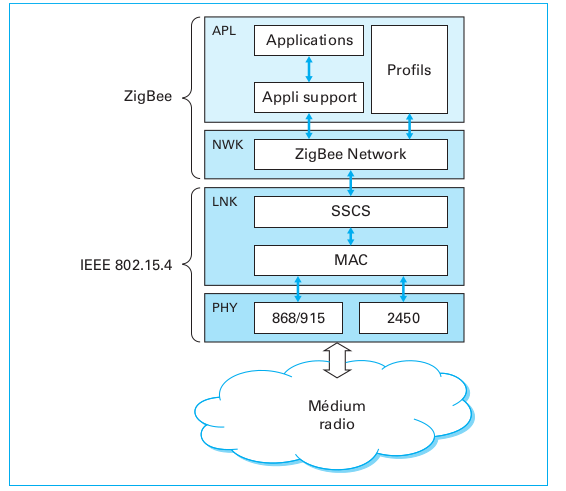
\includegraphics[scale=0.4]{OSI-Zigbee.png}
      \end{center}  
  \end{frame}

  \begin{frame}
    \frametitle{Comparatif}
    \begin{block}{Schema comparatif des différents protocole sans fil}
      \begin{center}
       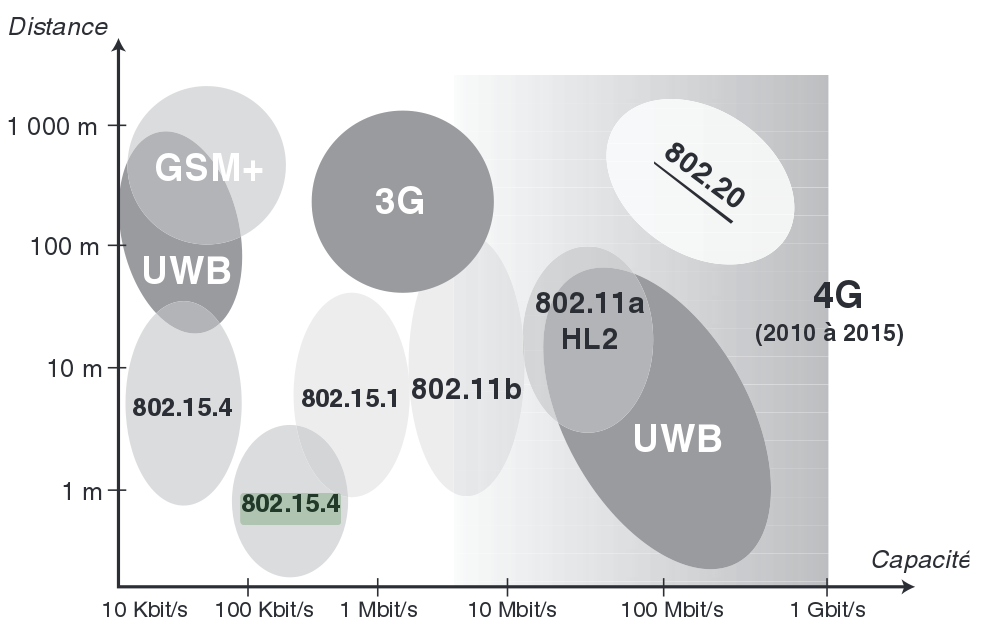
\includegraphics[scale=0.3]{Range.png}
      \end{center} 
    \end{block}
  \end{frame}
  
  \begin{frame}
    \frametitle{La couche physique}
    Contient l'émetteur/récepteur radio, avec un mécanisme de contrôle de qualité du signal et CCA
    \begin{block}{Débit}
      \begin{center}
       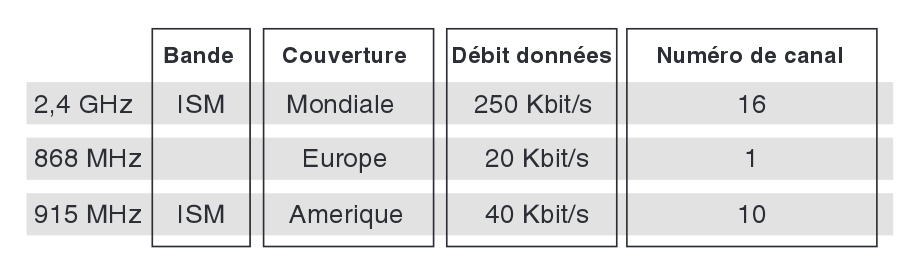
\includegraphics[scale=0.25]{Vitesse-Zigbee.png}
      \end{center}
    \end{block}
  \end{frame}
  
  \begin{frame}
    \frametitle{La couche d'accès au medium (MAC)}
    \begin{block}{Rôle des éléments du réseau}
      \begin{itemize}
        \item Le coordinateur (ZC) est le noeud principal, il est unique
        \item Les FFD ou routeurs gèrent le routage et les terminaux
        \item Les RFD ou terminaux sont de simple capteurs aux extremités du réseau
      \end{itemize}
    \end{block}
  \end{frame}
  
  \begin{frame}
    \frametitle{La couche d'accès au medium (MAC)}
    \begin{block}{Format de trame}
      \begin{itemize}
        \item En-tête (contrôle de trame, numéro de séquence, adressage)
        \item Données
        \item Pied (CRC)
        \begin{center}
         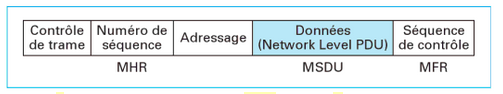
\includegraphics[scale=0.5]{Couche-MAC.png}
        \end{center} 
      \end{itemize}
    \end{block}
    \begin{block}{Il existe deux modes de fonctionnement}
      \begin{itemize}
        \item Le mode non-coordonnée
        \item Le mode coordonnée, ou balisé
      \end{itemize}
    \end{block}
  \end{frame}
  
  \begin{frame}
    \frametitle{La couche d'accès au medium (MAC)}
    \begin{block}{Le mode non-Coordonnée}
      \begin{itemize}
        \item Pas d'emission de \textit{beacon}
        \item Fonctionnement CSMA/CA pour gérer les collisions
        \item Le coordinateur est éveillé en permanence
      \end{itemize}
    \end{block}
  \end{frame}

  \begin{frame}
    \frametitle{La sous-couche d'accès au medium (MAC)}
    \begin{block}{Le mode Coordonnée}
      Le coordinateur diffuse périodiquement des \textit{beacon}. Tous les dispositifs sont informés de :
      \begin{itemize}
        \item La durée de la \textit{superframe} et quand ils peuvent transmettre des données en CSMA/CA
        \item A partir de quel moment le coordinateur rentre en hibernation et pour quelle durée
	\begin{center}
	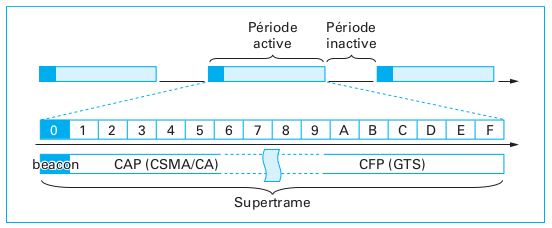
\includegraphics[scale=0.4]{Supertrame.png}
	\end{center} 
      \end{itemize}
    \end{block}
  \end{frame}

  \begin{frame}
    \frametitle{La sous-couche de convergence (LLC)}
    \begin{itemize}
      \item Vérification de l'intégrité des données reçues
      \item Contrôle de flux, afin d'éviter la saturation
      \item La convergence d'adressage (correspondance co uche 2 et 3 du modèle OSI, gestion du boradcast et en multicast)
    \end{itemize}
  \end{frame}

  \section{Les couches 4 à 7}
  \begin{frame}
    \frametitle{Présentation}
    \begin{itemize}
      \item 
      \item 
    \end{itemize}
    Example : 
    \begin{itemize}
      \item 
      \item 
    \end{itemize}
  \end{frame}

  \begin{frame}
    \frametitle{Adressage}
    \begin{itemize}
      \item Zigbee propose un algorithme de distribution d'adresses atomatique et décentralisé
      \item 
    \end{itemize}
    Example : 
    \begin{itemize}
      \item 
      \item 
    \end{itemize}
  \end{frame}

\section{Conclusion}
  \begin{frame}
  	\begin{block}{Zigbee est toujours le protocole de référence :}
	\begin{itemize}
		\item Porté par un consortium à la différence de Thread/Brillo (Google) Homekit (Apple) WeMo (Belkin), composé de Phillips/TexasInstrument/Schneider/NXP...
		\item Connu depuis longtemps d'où 75\% des parts de marché
		\item Possibilité pour les constructeurs de modifier les "profils Zigbee" i.e enrichir la couche applicative
		\item protocole en évolution constante : Zigbee 3.0 en développement
\end{itemize}  
\end{block}
\end{frame}
  

\begin{frame}
	  \begin{block}{Cependant quelques écueils qui pourraient se révéler graves}
	  \begin {itemize}
  \item Non compatible avec IP à la différence de 6LowPAN (sur lequel est basé Thread), ces protocoles devraient représenter 35\% des ventes en 2019 (2\% ajdh)
  \item une force est une faiblesse : pas d'entité unique qui porte le standard 
  \item de même les profils différents sont mal utilisés : amènent à des incompatibilités
  \item problèmes liés à la sécurité
\begin{itemize}
	\item Le réseau contient des noeuds à communication chiffrés, d'autres non, attque MiM
	\item Attaques restreintes (faible puissance de calcul)
	\item mais à venir !
\end{itemize}
  \end{itemize}
\end{block}
  \end{frame}

  

\end{document}
